\chapter{Interference}

\section{Preposition}

Two beam of light may interfere when:

\begin{itemize}
\item not perpendicular
\item has same frequency
\item has stable phase shift
\end{itemize}

\section{Algorithms}

Two wave of light $\vec{E}_1$ and $\vec{E}_2$

\begin{equation*}
  \begin{aligned}
    \vec{E}_1 = \vec{\varepsilon}_1 \exp \left[ i \left( \vec{k}_1 \cdot \vec{r} - \omega_1 t + \delta_1 \right) \right] \\
    \vec{E}_2 = \vec{\varepsilon}_2 \exp \left[ i \left( \vec{k}_2 \cdot \vec{r} - \omega_2 t + \delta_2 \right) \right]
  \end{aligned}
  \quad \Rightarrow \quad 
  \begin{aligned}
    I &= \left< \left| \left( \vec{E}_1 + \vec{E}_2 \right)^2 \right| \right> = \varepsilon_1^2 + \varepsilon_2^2 + 2 \vec{\varepsilon}_1 \cdot \vec{\varepsilon}_2 \cos \varphi \\
    \varphi &= \left( \vec{k}_2 \cdot r - \vec{k}_1 \cdot r \right) + \left( \omega_1 - \omega_2 \right) t + \left( \delta_2 - \delta_1 \right)
  \end{aligned}
\end{equation*}

\section{Young's Experiment}

\begin{figure}[H]
  \centering
  \begin{subfigure}{.55\textwidth}
    \centering
    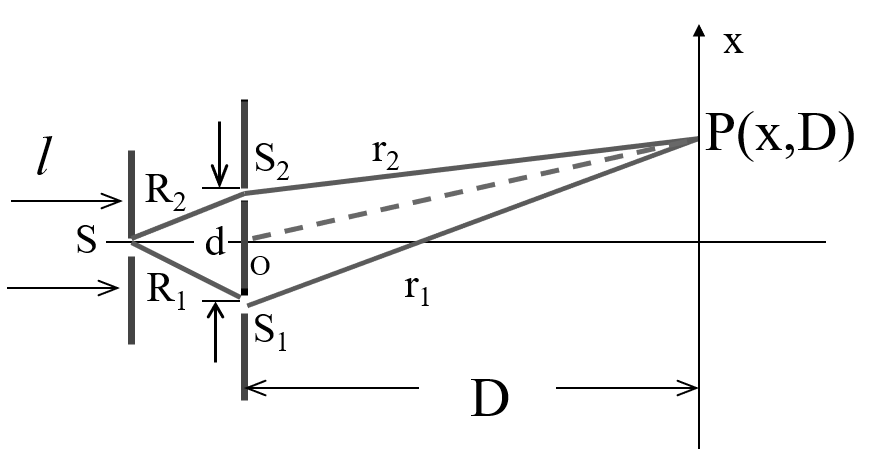
\includegraphics[width=\linewidth]{figures/Young-Exp}
  \end{subfigure}
  \begin{subfigure}{.35\textwidth}
    \centering
    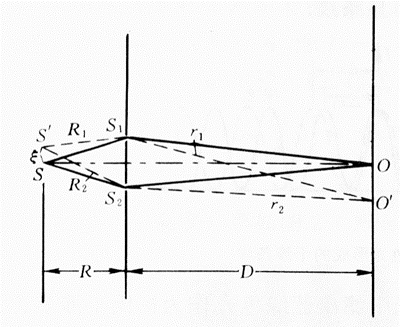
\includegraphics[width=\linewidth]{figures/Young-Exp-2}
  \end{subfigure}
\end{figure}

\begin{equation*}
  \begin{aligned}
    \Delta x = \dfrac{D}{d} \lambda 
  \end{aligned}
  \quad\quad 
  \begin{aligned}
    b \leq \lambda R \dfrac{1}{d} 
  \end{aligned}
  \quad\quad 
  \begin{aligned}
    I = 4 I_0 \cos^2 \left( \dfrac{d \pi}{D \lambda} x  \right) = 4 I_0 \cos^2 \left( \dfrac{\pi d \sin \theta}{\lambda}  \right)
  \end{aligned}
  \quad\quad 
  \begin{aligned}
    x_0 = - \dfrac{D}{R} \xi
  \end{aligned}
\end{equation*}

\section{Fresnel's Double Mirror}

\begin{figure}[H]
  \centering
  \includegraphics[width=0.9\linewidth]{figures/Fresnel-Double-Mirror}
\end{figure}

\begin{equation*}
  \begin{aligned}
    x_{white} = k \lambda \dfrac{D}{d} \quad\quad x_{black} = \dfrac{2 k + 1}{2} \lambda \dfrac{D}{d}   
  \end{aligned}
\end{equation*}

\section{Fresnel's Double Prism}

\begin{figure}[H]
  \centering
  \includegraphics[width=0.9\linewidth]{figures/Fresnel-double-prism}
\end{figure}

\begin{equation*}
  \begin{aligned}
    x_{white} = k \lambda \dfrac{D}{d} \quad\quad x_{black} = \dfrac{2 k + 1}{2} \lambda \dfrac{D}{d}   
  \end{aligned}
\end{equation*}

\section{Equal Inclination Interference}

\begin{figure}[H]
  \centering
  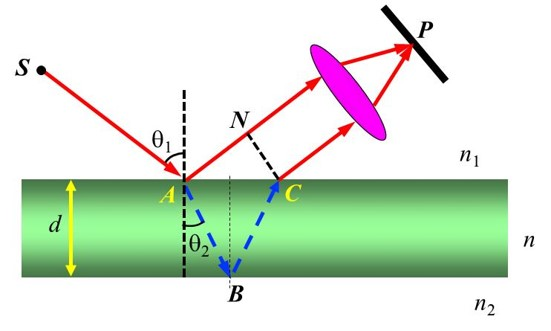
\includegraphics[width=0.4\linewidth]{figures/Equal-inclination}
\end{figure}

\begin{equation*}
  \begin{aligned}
    \Lambda =
  \end{aligned}
  \left\{
    \begin{aligned}
      & 2nk_0 d \cos \theta_2 \pm \pi && \quad\quad n_1 > n_2 < n_3 \ \text{OR} \  n_1 < n_2 > n_3 \\
      & 2nk_0 d \cos \theta_2 && \quad\quad n_1 < n_2 < n_3 \  \text{OR} \  n_1 > n_2 > n_3 \\
    \end{aligned}
  \right.
\end{equation*}

\section{Equal Thickness Interference}

\begin{figure}[H]
  \centering
  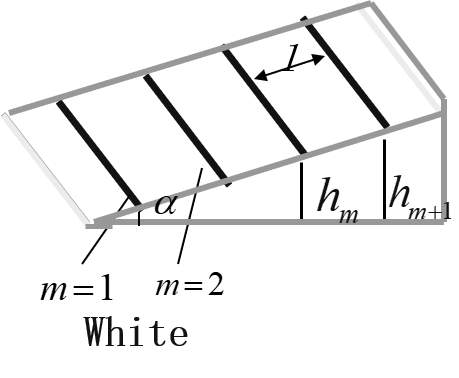
\includegraphics[width=0.4\linewidth]{figures/Equal-thickness}
\end{figure}

\begin{equation*}
  \begin{aligned}
    e = \Delta h = \dfrac{\lambda}{2 n} \quad\quad l = \dfrac{e}{\sin \alpha} = \dfrac{\lambda}{2 n \alpha} \approx \dfrac{\lambda}{2 n \alpha}   
  \end{aligned}
\end{equation*}

\section{Newton's Rings}

\begin{figure}[H]
  \centering
  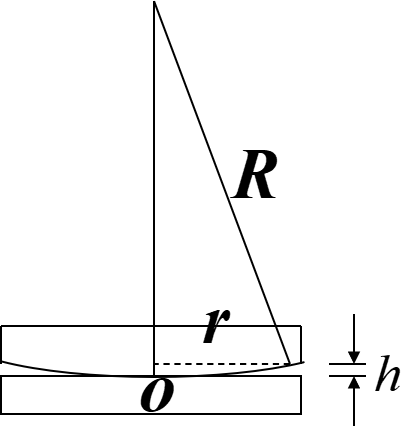
\includegraphics[width=0.4\linewidth]{figures/Newton-Ring}
\end{figure}

\begin{equation*}
  \begin{aligned}
    \Delta = 2 n h + \dfrac{\lambda}{2} = 
  \end{aligned}
  \left\{
    \begin{aligned}
      & k \lambda && \quad\quad \text{White} \\
      & \left( k + \dfrac{1}{2}  \right) \lambda && \quad\quad \text{Black}
    \end{aligned}
  \right.
\end{equation*}

\begin{equation*}
  \begin{aligned}
    h = R - \sqrt{R^2 - r^2} = R \left[ 1 - \sqrt{1 - \left( \dfrac{r}{R}  \right)^2 } \right] \approx \dfrac{r^2}{2R} 
  \end{aligned}
\end{equation*}

\begin{equation*}
  \begin{aligned}
    r^2 = 
  \end{aligned}
  \left\{
    \begin{aligned}
      & \left( k - \dfrac{1}{2}  \right) \dfrac{R \lambda}{n} && \quad\quad \text{White} \\
      & \dfrac{k R \lambda}{n} && \quad\quad \text{Black} 
    \end{aligned}
  \right.
\end{equation*}

\section{Double Beam F-P Interference}

\begin{minipage}[htbp]{0.4\linewidth}
  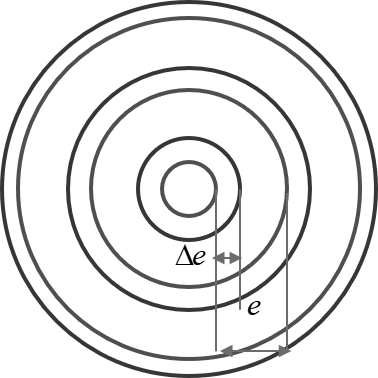
\includegraphics[width=\linewidth]{figures/double-beam-interference.png}
\end{minipage}
\begin{minipage}[htbp]{0.6\linewidth}
  \begin{equation*}
    \begin{aligned}
      & \left( m - \dfrac{\phi}{\pi}  \right) \lambda = 2 h \cos \theta_2 \\
      \\
      & \text{Same level, different wavelength} \\
      & \left( m - \dfrac{\phi}{\pi}  \right) \Delta \lambda = - 2 h \sin \theta_2 \Delta \theta_2 \approx - 2 h \theta_2 \Delta \theta_2 \\
      & \Delta e = f \Delta \theta_2 = - f \left( m - \dfrac{\phi}{\pi}  \right) \dfrac{\Delta \lambda}{2 h \theta_2} \\
      \\
      & \text{Same wavelength, different level} \\
      & \Delta m \lambda = - 2 h \sin \theta_2 \Delta \theta_2 \approx - 2 h \theta_2 \Delta \theta_2 \\
      & e = f \Delta \theta_2 = - f \dfrac{\lambda}{2 h \theta_2}  
    \end{aligned}
  \end{equation*}
\end{minipage}

Maximum wave length: 

\begin{equation*}
  \begin{aligned}
    \dfrac{\Delta e}{e} = \left( m - \dfrac{\phi}{\pi}  \right) \dfrac{\Delta \lambda}{\lambda} = 2 h \cos \theta_2 \dfrac{\Delta \lambda}{\lambda^2} \approx 2 h \dfrac{\Delta \lambda}{\lambda^2}
    \quad \Rightarrow \quad
    \Delta \lambda \approx \dfrac{\Delta e}{2 h e} \lambda^2
    \quad + \quad
    \Delta e = e
    \quad \Rightarrow \quad
    \left( \Delta \lambda \right)_{SR} = \dfrac{\lambda^2}{2h} 
  \end{aligned}
\end{equation*}

Minimum wavelength:

\begin{equation*}
  \begin{aligned}
    \dfrac{\lambda}{\Delta \lambda_{min}} = \dfrac{\pi m}{2} \sqrt{F}
    \quad\quad
    F = \dfrac{4 R}{\left( 1 - R \right)^2} 
  \end{aligned}
\end{equation*}

\section{Film}

\begin{figure}[H]
  \centering
  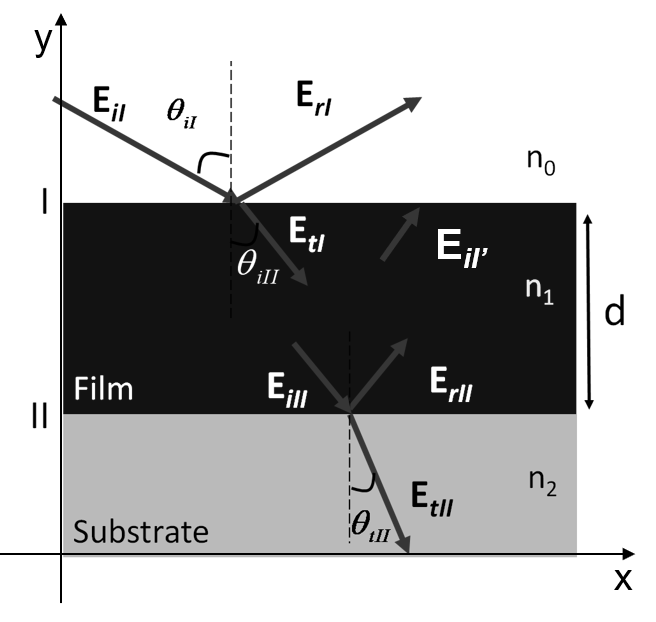
\includegraphics[width=0.5\linewidth]{figures/film.png}
\end{figure}

Phase shift

\begin{equation*}
  \Delta \phi = 
  \left\{
  \begin{aligned}
    & 2 d k_0 n_1 - 0 \quad\quad n_1 < n_2 \quad\quad \text{half wave loss happened in both of the 2 reflected wave}\\
    & 2 d k_0 n_1 - \pi \quad\quad n_1 > n_2 \quad\quad \text{half wave loss happened only once}
  \end{aligned}
  \right.
\end{equation*}

Reflective index

\begin{equation*}
  R = \left\{
  \begin{aligned}
    \left( \dfrac{n_0 n_2 - n_1^2}{n_0 n_2 + n_1^2}  \right)^2 & \quad\quad n_1 < n_2 \\
    \left( \dfrac{n_0 - n_2}{n_0 + n_2}  \right)^2 & \quad\quad n_1 > n_2 
  \end{aligned}
  \right.
\end{equation*}

\section{Grating}

\begin{figure}[H]
  \centering
  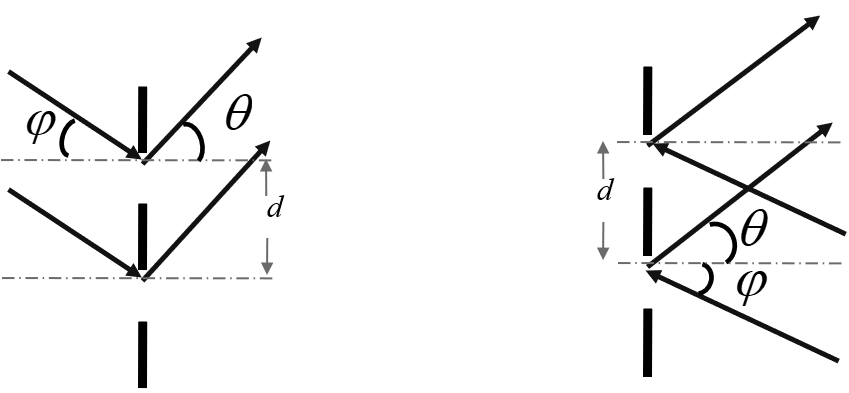
\includegraphics[width=0.9\linewidth]{figures/grating.png}
\end{figure}


%%% Local Variables:
%%% mode: latex
%%% TeX-master: "Optics"
%%% End:
